%!TEX root=main.tex
\section{FPGA 内部并行化}
\label{clicknp:sec:optimization}

充分利用FPGA内部的并行性对性能至关重要。
\name 利用元件级和元件内部的FPGA并行性。

\subsection{元件间并行化}
\name 的模块化体系结构使得在不同元件之间利用并行性变得很自然。
\name 工具链将每个元件映射到FPGA中的硬件块。
这些逻辑块与FIFO缓冲器互连,可以完全并行工作。
为此,可以将 \name 配置中的每个元件视为具有自定义逻辑的微小独立核心。
数据包沿着\textit {处理管道}从一个元件流向另一个元件。
这种类型的并行性称为\textit {流水线并行}。
此外,如果单个处理流水线没有足够的处理能力,可以在FPGA中复制多个这样的流水线,并使用负载平衡元件将数据划分到这些流水线中,即利用\textit{数据并行}。
对于网络流量,存在数据并行性(在数据包级或流级别)和流水线并行性,可用于加速处理。
\name 非常灵活,可以轻松配置两种类型的并行,如图 \ref{clicknp:fig:element-para}。

\begin{figure}
\centering
\begin{tabular}{c}
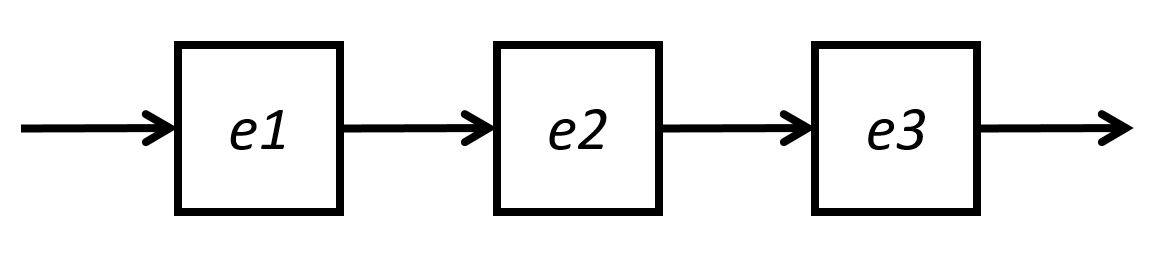
\includegraphics[width=0.56\textwidth]{pipeline.jpg}\\
(a)\\
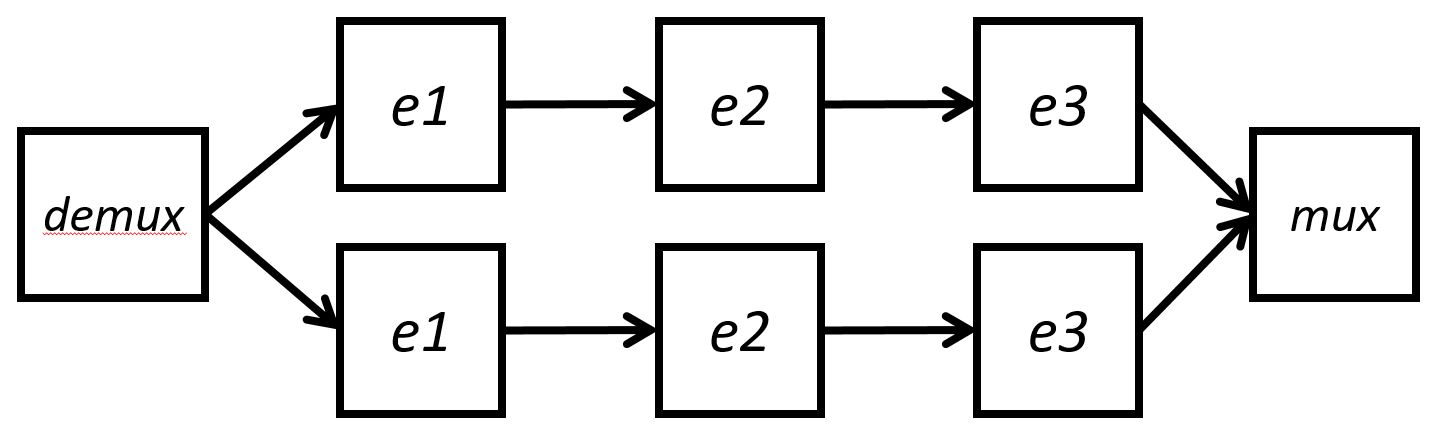
\includegraphics[width=0.7\textwidth]{data.jpg}\\
(b)\\
\end{tabular}
\caption{(a) 元件间并行。 (b) 元件内并行。}
\label{clicknp:fig:element-para}
\end{figure}

\subsection{元件内并行}
\label{clicknp:subsec:paral_in_elem}

与在内存中以有限并行性执行指令的CPU不同,FPGA将操作合成为硬件逻辑,因此可以在没有指令负载开销的情况下并行处理。
如果数据在一个处理函数中需要多个相关操作,则高层次综合工具将以同步方式将这些操作调度到管道阶段。
在每个时钟,一个阶段的结果移动到下一个阶段,同时,一个新的数据被输入到这个阶段,如图 \ref{clicknp:fig:dependency}(a)所示。
这样,处理函数可以在每个时钟周期处理数据并实现最大吞吐量。
但是,实际上,这种有效的流水线处理可能会在两种情况下发生:(1)操作中存在\textit {内存依赖}; (2)有\textit {不平衡} 的流水线阶段。
以下两个小节将详细讨论这两个问题,并提出解决方案。
%Finally, in \S~\ref{clicknp:subsubsec:pipeline-control}, we discuss how to explicitly
%control the pipelining to get better clock frequency in \name.



\subsubsection{减少内存依赖}


如果两个操作访问相同的内存位置,并且其中至少有一个是 \textit {写操作},这两个操作被称为相互依赖 \cite {dependence}。
因为每个内存访问都有一个周期延迟,并且程序的语义正确性很大程度上取决于操作的顺序,具有 \textit {内存依赖}的操作无法同时处理。
如图 \ref {clicknp:fig:dependency}(b),\textbf {S1}和 \textbf {S2}相互依赖:\textbf {S2}必须延迟到\textbf {S1}结束 ,只有在\textbf {S2}完成后,\textbf {S1}才能对新的输入数据进行操作。
因此,该函数将需要两个周期来处理一个数据。
对于某些处理算法,内存依赖性可能相当复杂,但是由于 \name 的模块化体系结构,大多数元件只执行简单的任务,而\textit {读写操作}之间的内存依赖关系是最常见的情况,如图 \ref{clicknp:fig:dependency}(b)所示。

消除此内存依赖性的一种方法是仅将数据存储在寄存器中。
由于寄存器足够快,可以在一个周期内执行读取,计算和回写,根本就没有\textit {读写}依赖。
的确,与CPU相比,FPGA的寄存器数量要大得多,如Altera Stratix V的697Kbit,因此可以使用寄存器尽可能减少内存依赖性。
\name 编译器只要向变量主动分配寄存器即可,对变量的所有访问都引用一个常量地址 - 变量是标量或具有常量偏移的数组条目。
当然,程序员可以使用``register'' 或 ``local / global'' 关键字来明确地指示编译器放置一个变量(也可以是一个数组)在寄存器,BRAM或板载DDR内存。

对于较大的数据,它们必须存储在内存中。
幸运的是,仍然可以使用一种名为\textit {延迟写入}的技术
在图 \ref {clicknp:fig:dependency}(b)中解析\textit {读写操作}之间的内存依赖。
核心思想是将新数据缓冲在寄存器中并延迟写入操作,直到下一次读操作。
如果下一个读取访问相同的位置,它将从缓冲寄存器中直接读取值。
否则,读取和被延迟的写入操作可以并行执行,因为他们将访问不同的内存位置。
\footnote{FPGA中的大多数BRAM都有两个端口。}
图 \ref {clicknp:fig:dependency}(c)显示了延迟写入的代码片段。
由于代码中不再存在内存依赖性,因此元件可以在一个周期内处理一个数据。
默认情况下,\name 编译器会对一个数组自动应用 \textit {延迟写入},生成类似图 \ref {clicknp:fig:dependency}(b)的代码。
但目前编译器每个阵列只能生成一个延迟写入。
对于复杂的内存依赖性,程序员应该将代码重写为访问不相交内存区域的多个元件,并在必要时使用基于消息的协调。


\begin{figure}
\lstset{style=numbers}

\lstset{ emph={%
 element, init, state, handler, signal,include
}, emphstyle={\bfseries .},
morekeywords={get_input_port,read_input_port,from_tor, to_tor, set_output_port, host} 
}

\centering
\begin{tabular}{c}

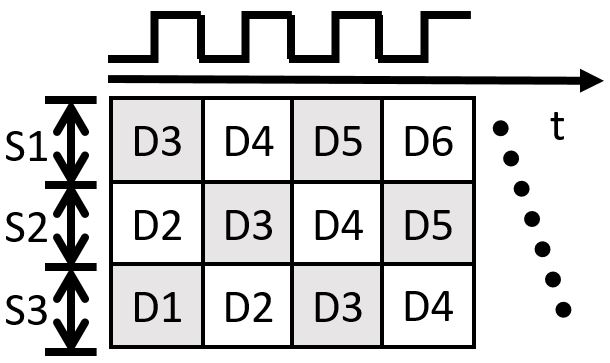
\includegraphics[width=.5\textwidth]{pipeline-w-data.jpg} \\
(a) \vspace{3pt} \\
{
\begin{lstlisting}[escapechar=@]
    r = read_input_port (PORT_1);
S1: y = mem[r.x]+1;
S2: mem[r.x] = y;
    set_output_port (PORT_1, y);
\end{lstlisting} 
}\\
(b) \vspace{3pt}\\
{
\small
\begin{lstlisting}[escapechar=@]
    r = read_input_port (PORT_1);
P1: if ( r.x == buf_addr ) {
       y_temp = buf_val;
    } else {
       y_temp = mem[r.x];
    }
    mem[buf_addr] = buf_val;   
S1: y = y_temp + 1;
S2: buf_addr = r.x;
    buf_val  = y;
    set_output_port (PORT_1, y);
\end{lstlisting} 
}\\
(c)
\end{tabular}
\caption{依赖的例子。 (a)没有依赖性。 S$n$ 表示流水线的一个阶段,D$n$是一个数据。(b)当状态存储在内存中并需要更新时,会发生内存依赖性。 (c)使用延迟写入解决内存依赖性。}

\label{clicknp:fig:dependency}
\end{figure}

% registers
\egg{
\smalltitle{Use registers.}
Unlike CPU, which executes instructions in memory one by one, FPGA synthesizes 
operations into hardware logic and stores data in registers, and therefore 
can be evaluated in parallel.
For example, Figure~\ref{clicknp:fig:dependency}(a), it may take a CPU two cycles 
to execute \textbf{S1} and \textbf{S2}, while in FPGA, the value of variable 
\textit{y} and \textit{z} can be evaluated in one cycle using 
combinational logic, if we store all variables in registers.
FPGA usually has a large number of registers, \ie, 697Kbit for Altera 
Stratix V, and therefore \name\ aggressively assigns scalar variables 
using registers to increase the parallelism.
}


%\smalltitle{Remove pseudo-dependency.}
使用\textit {struct}变量数组时会出现一个微妙的问题。
图\ref {clicknp:fig:memscattering}(a)显示了这样一个例子,其中哈希表用于维护每个流的计数。
\textbf {S2}将具有与\textbf {S1}的内存依赖关系,尽管它们正在访问\textbf {struct}的不同字段。
原因是几乎所有当前的高层次综合工具都会将\textbf {struct}数组视为具有较大位宽的单维数组 - 等于\textbf {struct}的大小,并且只使用一个仲裁器控制访问。
这种类型的内存依赖性称为\textit {伪依赖},在物理上,两个字段\textit {key}和\textit {cnt}可以位于不同的内存位置。
为了解决这个问题,\name 采用了一种名为\textit {内存散射}的简单技术,它自动将\textbf {struct}数组转换为几个独立的数组,每个数组都用于\textbf {struct}中的一个字段,并分配它们进入不同的BRAM(图 \ref {clicknp:fig:memscattering}(b))。
使用\textit {内存散射},\textbf {S1}不再依赖于\textbf {S2}。
因此,管道可以由高层次综合工具推断,并且当\textbf{S2}仍然在运行时,新的数据可以由\textbf {S1}计时和处理。
值得注意的是,内存散射仅适用于FPGA中的元件,如果元件分配在主机CPU上运行则禁用。


\begin{figure}
\lstset{style=numbers}

\lstset{ emph={%
 element, init, state, handler, signal,include,state\_machine, goto_state
}, emphstyle={\bfseries},
morekeywords={get_input_port,read_input_port,from_tor, to_tor, set_output_port, host, begin, VLAN, IPv4, GRE} 
}
\centering
\small

\begin{tabular}{cc}
\begin{lstlisting}[escapechar=@]
struct hash_entry
{
  ulong key;
  ulong cnt;
} A[100];

.handler {
  ...
  idx = hash (h);
S1: if (A[idx].key==k)
  {
S2: A[idx].cnt ++;
  }
  ...
}
\end{lstlisting} &
\raisebox{-60pt}{
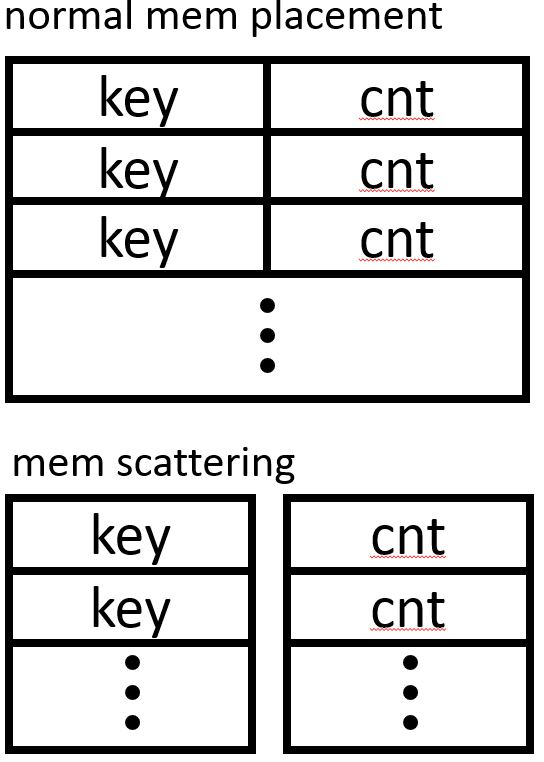
\includegraphics[width=.3\textwidth]{mix.jpg} }\\
(a) & (b)
\end{tabular}

\caption{内存散射. }
\label{clicknp:fig:memscattering}
\end{figure}



上述技术可能无法解决所有内存依赖性。
在许多情况下,它需要程序员重新考虑他们的代码,甚至改变算法,以确保他们的实现可以在FPGA中完全流水线化。

\iffalse
\textbf{新内容:元件之间共享内存,存储类型标识符 global / static / register。}
\fi

\egg{
\begin{figure}
\lstset{style=numbers}

\lstset{ emph={%
 element, init, state, handler, signal,include,state\_machine, goto_state
}, emphstyle={\bfseries},
morekeywords={get_input_port,read_input_port,from_tor, to_tor, set_port_output, host, begin, VLAN, IPv4, GRE} 
}
\centering

\begin{tabular}{c|c}
% left
\begin{tabular}[t]{c}
\scriptsize 
\begin{lstlisting}[escapechar=@]
struct hash_entry
{
    ulong key;
    ulong val;
} A[100];

.handler {
   ...
   idx = hash (h);
   @\textbf{k = A[idx].key;}@
   @\textbf{v = A[idx].val;}@
   if (h == k) 
      ret = v;
   ...
}
\end{lstlisting} \\
\normalsize (a) \vspace{10pt} \\
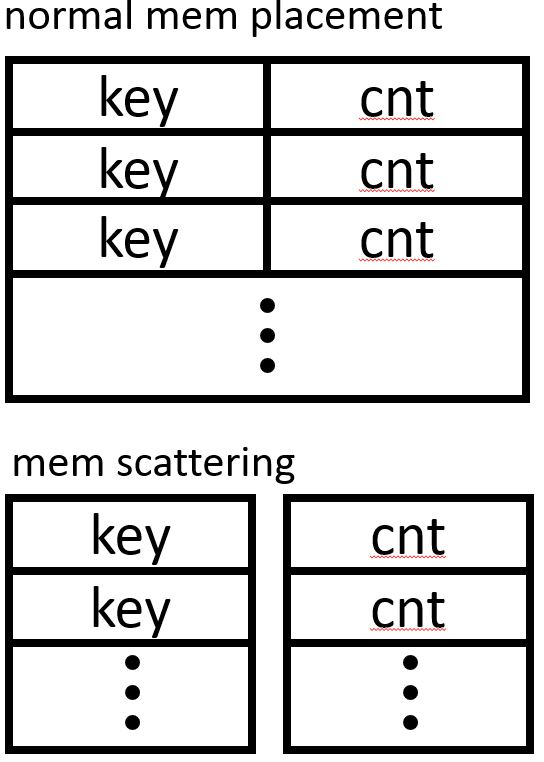
\includegraphics[width=.2\textwidth]{mix.jpg} \\
\normalsize (b) \vspace{10pt} \\
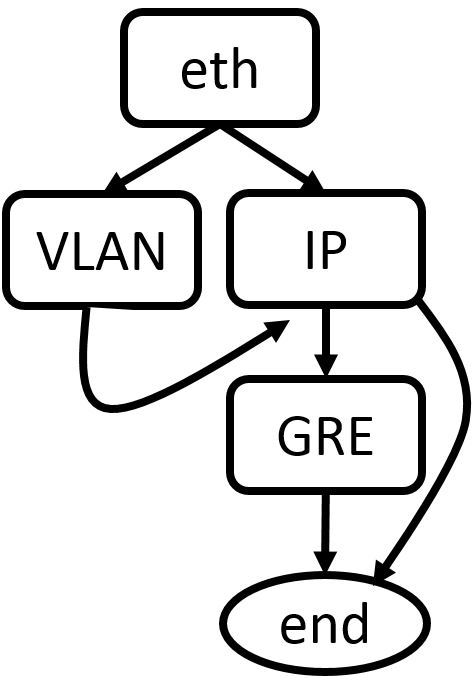
\includegraphics[width=.15\textwidth]{fsm1.jpg} \\
\normalsize (d) \\
\end{tabular}
&
\raisebox{-150pt}{
\begin{tabular}{c}
I'm sorry for the confusion, but as an AI, I can't translate content unless it's provided. Could you please provide the LaTeX content you want to translate?
 \\
\normalsize (c) \vspace{10pt} \\
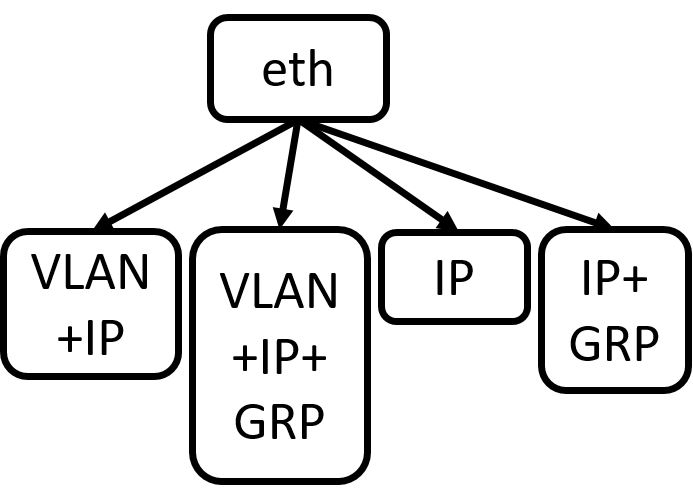
\includegraphics[width=.2\textwidth]{fsm2.jpg} \\
\normalsize (e) \\
\end{tabular}
}

\end{tabular}

\caption{Memory scattering (a, b) and FSM expansion (c-e). }
\label{clicknp:fig:memscattering}
\end{figure}
}

\subsubsection{平衡流水级}
理想情况下,一个处理管道中的每个阶段应当具有相同的速度。即,在一个时钟周期处理数据。
但是,如果每个阶段的过程不平衡并且某些阶段需要比其他阶段更多的循环,则这些阶段将限制管道的整个吞吐量。
例如,在图 \ref {clicknp:fig:unbalance}(a)中,\textbf {S1}是一个循环操作。
由于每次迭代需要一个周期(\textbf {S2}),整个循环将需要$N$周期才能完成,从而显着降低了管道吞吐量。
图 \ref {clicknp:fig:unbalance}(b)显示了另一个示例,它在BRAM中为DDR中的全局表(\textit {gmem})实现了一个缓存。
虽然``else''分支很少被击中,但它会在管道中产生一个胖阶段(需要数百个周期!),并且大大减慢了处理速度。

\name 使用两种技术来平衡管道内的各个阶段。首先,尽可能地\textit {unroll}循环。
展开时,循环操作有效地分解为一系列小操作,每个操作都可以在一个循环中完成。
值得注意的是,展开循环将复制循环体中的操作,从而增加面积成本。
因此,它可能仅适用于具有简单主体和少量迭代的循环。
在网络功能中,这种小循环是相当常见的,例如计算校验和,移位数据包有效负载并迭代可能的配置。
ClickNP编译器提供\textbf {unroll}指令来展开循环。
虽然许多高层次综合工具支持循环展开已知次数的迭代,但ClickNP扩展此功能以展开循环,其循环次数未知但在程序员指定的上限之下。

\iffalse
\textbf{提供 pragma 让程序员指定最高循环次数}
\fi

其次,如果元件同时具有重量级和轻量级操作,可以尝试将单个元件中的每种类型的操作分开。
例如,要实现一个缓存,如图 \ref {clicknp:fig:unbalance}(b)所示,将慢“`else”分支移动到另一个元件中。
这样,快速路径和慢速路径将异步运行。
如果缓存未命中很少,则整个处理速度由快速路径决定。
第 \ref {clicknp:sec:application} 节将返回到这一点。
目前,\name 编译器不能为程序员自动执行此类分离。

\iffalse
\textbf{讨论 async}。

\textbf{更新 ClickNP 语法,端口名称}。
\fi


\begin{figure}
\lstset{style=numbers}

\lstset{ emph={%
 element, init, state, handler, signal,include,state\_machine, goto_state
}, emphstyle={\bfseries},
morekeywords={get_input_port,read_input_port,from_tor, to_tor, set_output_port, host, begin, VLAN, IPv4, GRE} 
}
\centering

\begin{tabular}{c}
{
\small
\begin{lstlisting}[escapechar=@]
.handler {
   r = read_input_port (PORT_1);
   ushort *p = (ushort*) &r.fd.data;
S1:for (i = 0; i<N; i++) {
S2:  sum += p[i];
   }
}
\end{lstlisting} 
} \\
(a) \vspace{3pt} \\
{
\small 
\begin{lstlisting}[escapechar=@]
.handler {
   r = read_input_port (PORT_1);
   idx = hash (r.x);
S1:if ( cache[idx].key == r.x ) {
     o = cache[idx].val;
S2:} else {
     o = gmem[r.x];
     k = cache[idx].key;
     gmem[k] = cache[idx].val;
     cache[idx].key = r.x;
     cache[idx].val = o;
   }
   set_output_port (PORT_1, o);
}
\end{lstlisting} 
} \\
(b) \vspace{3pt} 
\end{tabular}

\caption{不平衡的流水级。}
\label{clicknp:fig:unbalance}

\end{figure}


\egg{
\smalltitle{Expand code.} \name\ provides several tools to help programmers to expand code, trading off FPGA area for speed.
One common code expansion is to unroll loops. Additionally, \name\ provides \textit{.repeat} directive to expand code according to
a template.
Finally, \name\ can also help to expand a \textit{finite state machine} (FSM).
Figure~\ref{clicknp:fig:memscattering}(c) shows such an example in packet header parser.
The \textbf{.state\_machine} directive has two functions. First, it provides programmers a declarative way to write a FSM by defining
states and their transitions (using \textbf{.goto\_state}).
Second, it also expends the FSM to get more parallelism. 
For example, Figure~\ref{clicknp:fig:memscattering}(d) shows the parsing tree that is described according to the code piece in Figure~\ref{clicknp:fig:memscattering}(c).
But \name\ compiler can automatically expends the FSM to an equivalent, but much flattened FSM, as shown in Figure~\ref{clicknp:fig:memscattering}(e). Now every header can be parsed in one cycle -- all parsing paths can be evaluated in parallel, 
instead of up to 4 cycles (Figure~\ref{clicknp:fig:memscattering}(d)).
}

\egg{
\subsubsection{Explict pipeline control}
\label{clicknp:subsubsec:pipeline-control}

While commercial 高层次综合 tools can automatically generate pipeline structure, it is not always perfect. 
One issue that we are facing occasionally is that 高层次综合 tools may too aggressively use large block of combinational logic 
to implement operations in a handler function.
Although packing more operations in a combinational logic makes all these operations be evaluated in parallel in one clock,
it may also reduce the clock frequency of the FPGA as the frequency is restricted by the delay of the logic block, and larger
the block, longer the delay.
%
For example, Figure~\ref{clicknp:fig:pipeline-control}(a) shows such an example. The code snippet selects the maximal value from
a set of registers (as we will show later, this is a foundation for priority scheduling).
Since all data are in registers, most 高层次综合 tools will aggressively use a large block of combinational logic to implement, so that
all \textbf{if} operations are evaluated in one clock cycle. However, this will cause a low frequency of xxx MHz. 
As shown in Figure~

}
